\documentclass{article}
\usepackage{amsmath}
\usepackage{graphicx}
\begin{document}
\begin{center}
\textbf{QUADRATIC EQUATIONS}
\end{center}
\begin{enumerate}
	\item Find the value of $p$ for which one root of the quadratic equation \\ $( px^2-14x+8=0$) is $6$ times the other
\end{enumerate}
\begin{center}
\textbf{TRIGNOMETRY}
\end{center}
\begin{enumerate}
	\item If a tower $30m$ high,casts a shadow of $(10\sqrt{3})m$ long on the ground, \\ then what is the angle of elevation of the sun?
	\item On a straight line passing through the foot of a tower, two points $C$ and $D$ are at distances of $4m$ and $16m$ from the foot respectively. If the angles of elevation from $C$ and $D$ of the top of the tower are complementary, then find the height of the tower.
\end{enumerate}
\begin{center}
\textbf{CIRCLES}
\end{center}
\begin{enumerate}
	\item If the angle between two tangents drawn from an external point $P$ to a circle of radius a and centre $O$, is $60^\circ $ then find the length of $OP$.
	\item $A$ circle touches all the four sides of a quadrilateral $ABCD$. Prove that\\
$AB + CD = BC + DA$
\item Prove that the tangents drawn at the end points of a chord of a circle make equal angles with the chord.
\end{enumerate}
\begin{center}
\textbf{PROGRESSIONS}
\end{center}
\begin{enumerate}
	\item What is the common difference of an A.P in which $(a_{21} - a_{7} = 84$)?
	\item For what value of $(n$), are the $(n)th$ terms of two A.Ps $(63,65,67, \dots$) and $(3, 10, 17, \dots$) equal?
	\item How many terms of an A.P. $9$, $17$, $25$, ... must be taken to give a sum of $636$?
\end{enumerate}
\begin{center}
\textbf{VOLUME \&\ SURFACE AREAS}
\end{center}
\begin{enumerate}
	\item The dimensions of a solid iron cuboid are \(4·4m \times 2·6m \times 1·0m\). It is  \\
melted and recast into a hollow cylindrical pipe of $30$ cm inner radius and \\
thickness $5$ cm. Find the length of the pipe.
\item A toy is in the form of a cone of radius $3·5cm$ mounted on a hemisphere \\
of same radius on its circular face. The total height of the toy is $15·5cm$. \\ 
Find the total surface area of the toy.
\end{enumerate}
\begin{center}
	\textbf{PROBABILITY}
\end{center}
\begin{enumerate}
	\item The probability of selecting a rotten apple randomly from a heap of $900$ \\ apples is $0.18$. What is the number of rotten apples in the heap?
	\item A bag contains $15$ white and some black balls. If the probability of \\ drawing a black ball from the bag is thrice that of drawing a white ball, \\ find the number of black balls in the bag.
\end{enumerate}
\begin{center}
\textbf{COORDINATE GEOMETRY}
\end{center}
\begin{enumerate}
\item A line intersects the y-axis and x-axis at the points $P$ and $Q$ respectively.\\
 If $(2,-5)$ is the mid-point of $PQ$, then find the coordinates of $P$ and $Q$.
 \item If the distances of $P(x, y)$ from $A(5, 1)$ and$B(-1, 5)$ are equal, then prove \\that $3x$ = $2y$.
 \item In what ratio does the point $[\frac{24}{11}, y]$ divide the line segment joining the \\ points P(2,-2) and Q(3,7)? Also find the value of y.
 \item Water in a canal, $5·4 m$ wide and $1·8 m$ deep,is flowing with a speed of \\ $25 km/hour$. How much area can it irrigate in $40 minutes$, if $10cm$ of \\standing water is required for irrigation ?                    
 \item Three semicircles each of diameter $3 cm$, a circle of diameter $4·5 cm$ and a semicircle of radius $4·5 cm$ are drawn in the given figure. Find the area of \\the shaded region.
 \begin{figure}[h!]
 \centering                 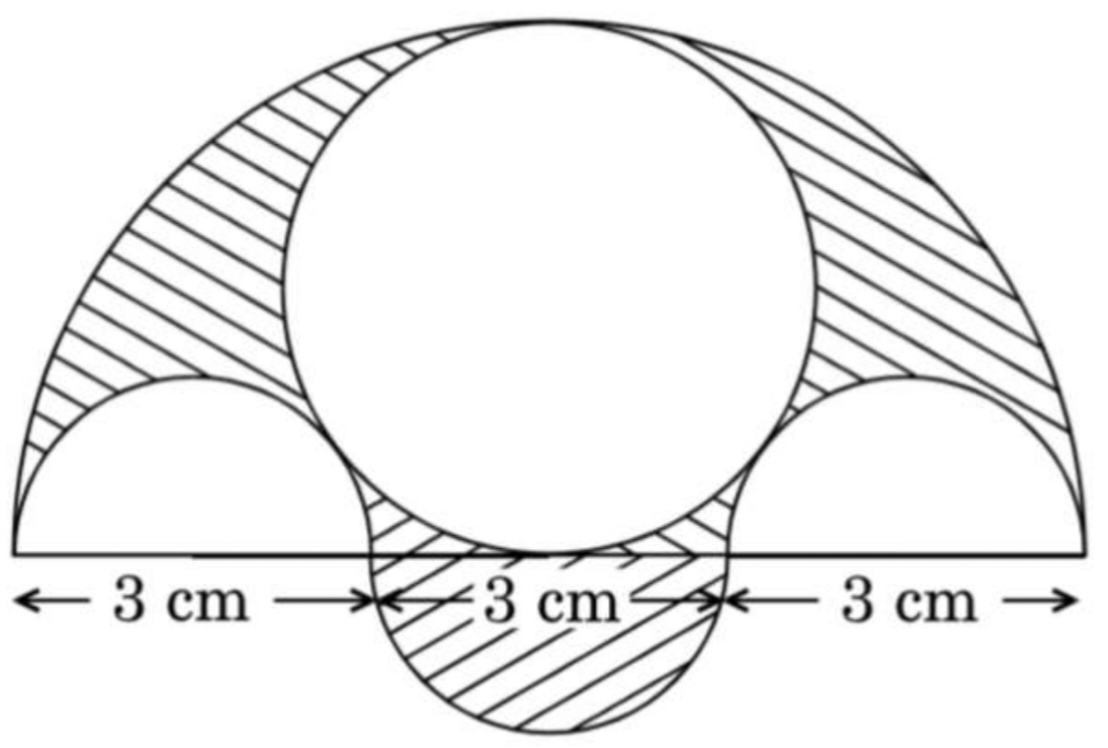
\includegraphics[width=0.75\textwidth]{compressed13.jpg}
 \end{figure}
 \item In the given figure, two concentric circles with centre $O$ have radii $21 cm$ \\
 20 and $42 cm$. If $ \angle AOB = 60^\circ $. find the area of the shaded region.
 \begin{figure}[h!]
 \centering
 \includegraphics[width=0.75\textwidth]{compressed16.jpg}
 \end{figure}
 \end{enumerate}

\end{document}
